\documentclass[11pt,a4paper]{article}
\usepackage[utf8]{inputenc}
\usepackage[bulgarian]{babel}
\usepackage{fullpage}
\usepackage{graphicx}
\usepackage{indentfirst}
\usepackage{hyperref}
\usepackage{xcolor}

\hypersetup{
    colorlinks,
    linkcolor={blue!55!black},
    citecolor={blue!50!black},
    urlcolor={blue!80!black}
}

\begin{document}
\linespread{1.25}
\begin{titlepage}
   \begin{center}
       \vspace*{1cm}

\LARGE
       \textbf{Софийски университет „Св. Климент Охридски“\\
       Факултет по математика и инфоратика\\}

 

\addvspace{110pt}


	\Huge
       \textbf{Проект по Бази данни}

	
       \vspace{0.5cm}
	\LARGE
        \textbf{Тема:} Библиотека
 
       \vspace{1.5cm}
   \end{center}
    \vfill
\Large
       \textbf{Съставил:\\Ростислав Стоянов\\ф-н 45244}
 
    
 
 
       \vspace{0.8cm}
 


 

\end{titlepage}

\large
\tableofcontents
\pagebreak


\section{Описание}
Всяка библиотека има клонове. Всеки клон се описва с уникален номер, име и адрес. Във всеки клон работят различни служители - всеки от тях се описва с ЕГН, име и позиция. Служителите могат да заемат различни позиции, като всеки служител работи в определен клон и си има ръководител (освен ръководителя на библиотеката). Във всеки клон на библиотеката се съхраняват книги, като в различните клонове може да се съхраняват различни книги, а една и съща книга може да бъде намерена на повече от едно място. Атрибутите, описващи една книга са: ISBN, име, автор, издателство, година на издаване, издание, страници, системен номер, тип. Издателствата се характеризират с индивидуален номер, име и адрес. Книгите могат да бъдат заемани за определен период (ако са налични) от граждани. Ако книгата не се върне в посочения срок, се начислява глоба. Гражданите се описват с ЕГН и име.
\pagebreak

\section{E\textbackslash R модел} 
E\textbackslash R модел, илюстриращ база данни, спазваща изискванията от описанието, е представен на следната диаграма: 
\begin{figure}[h!]
\hspace{-70pt}
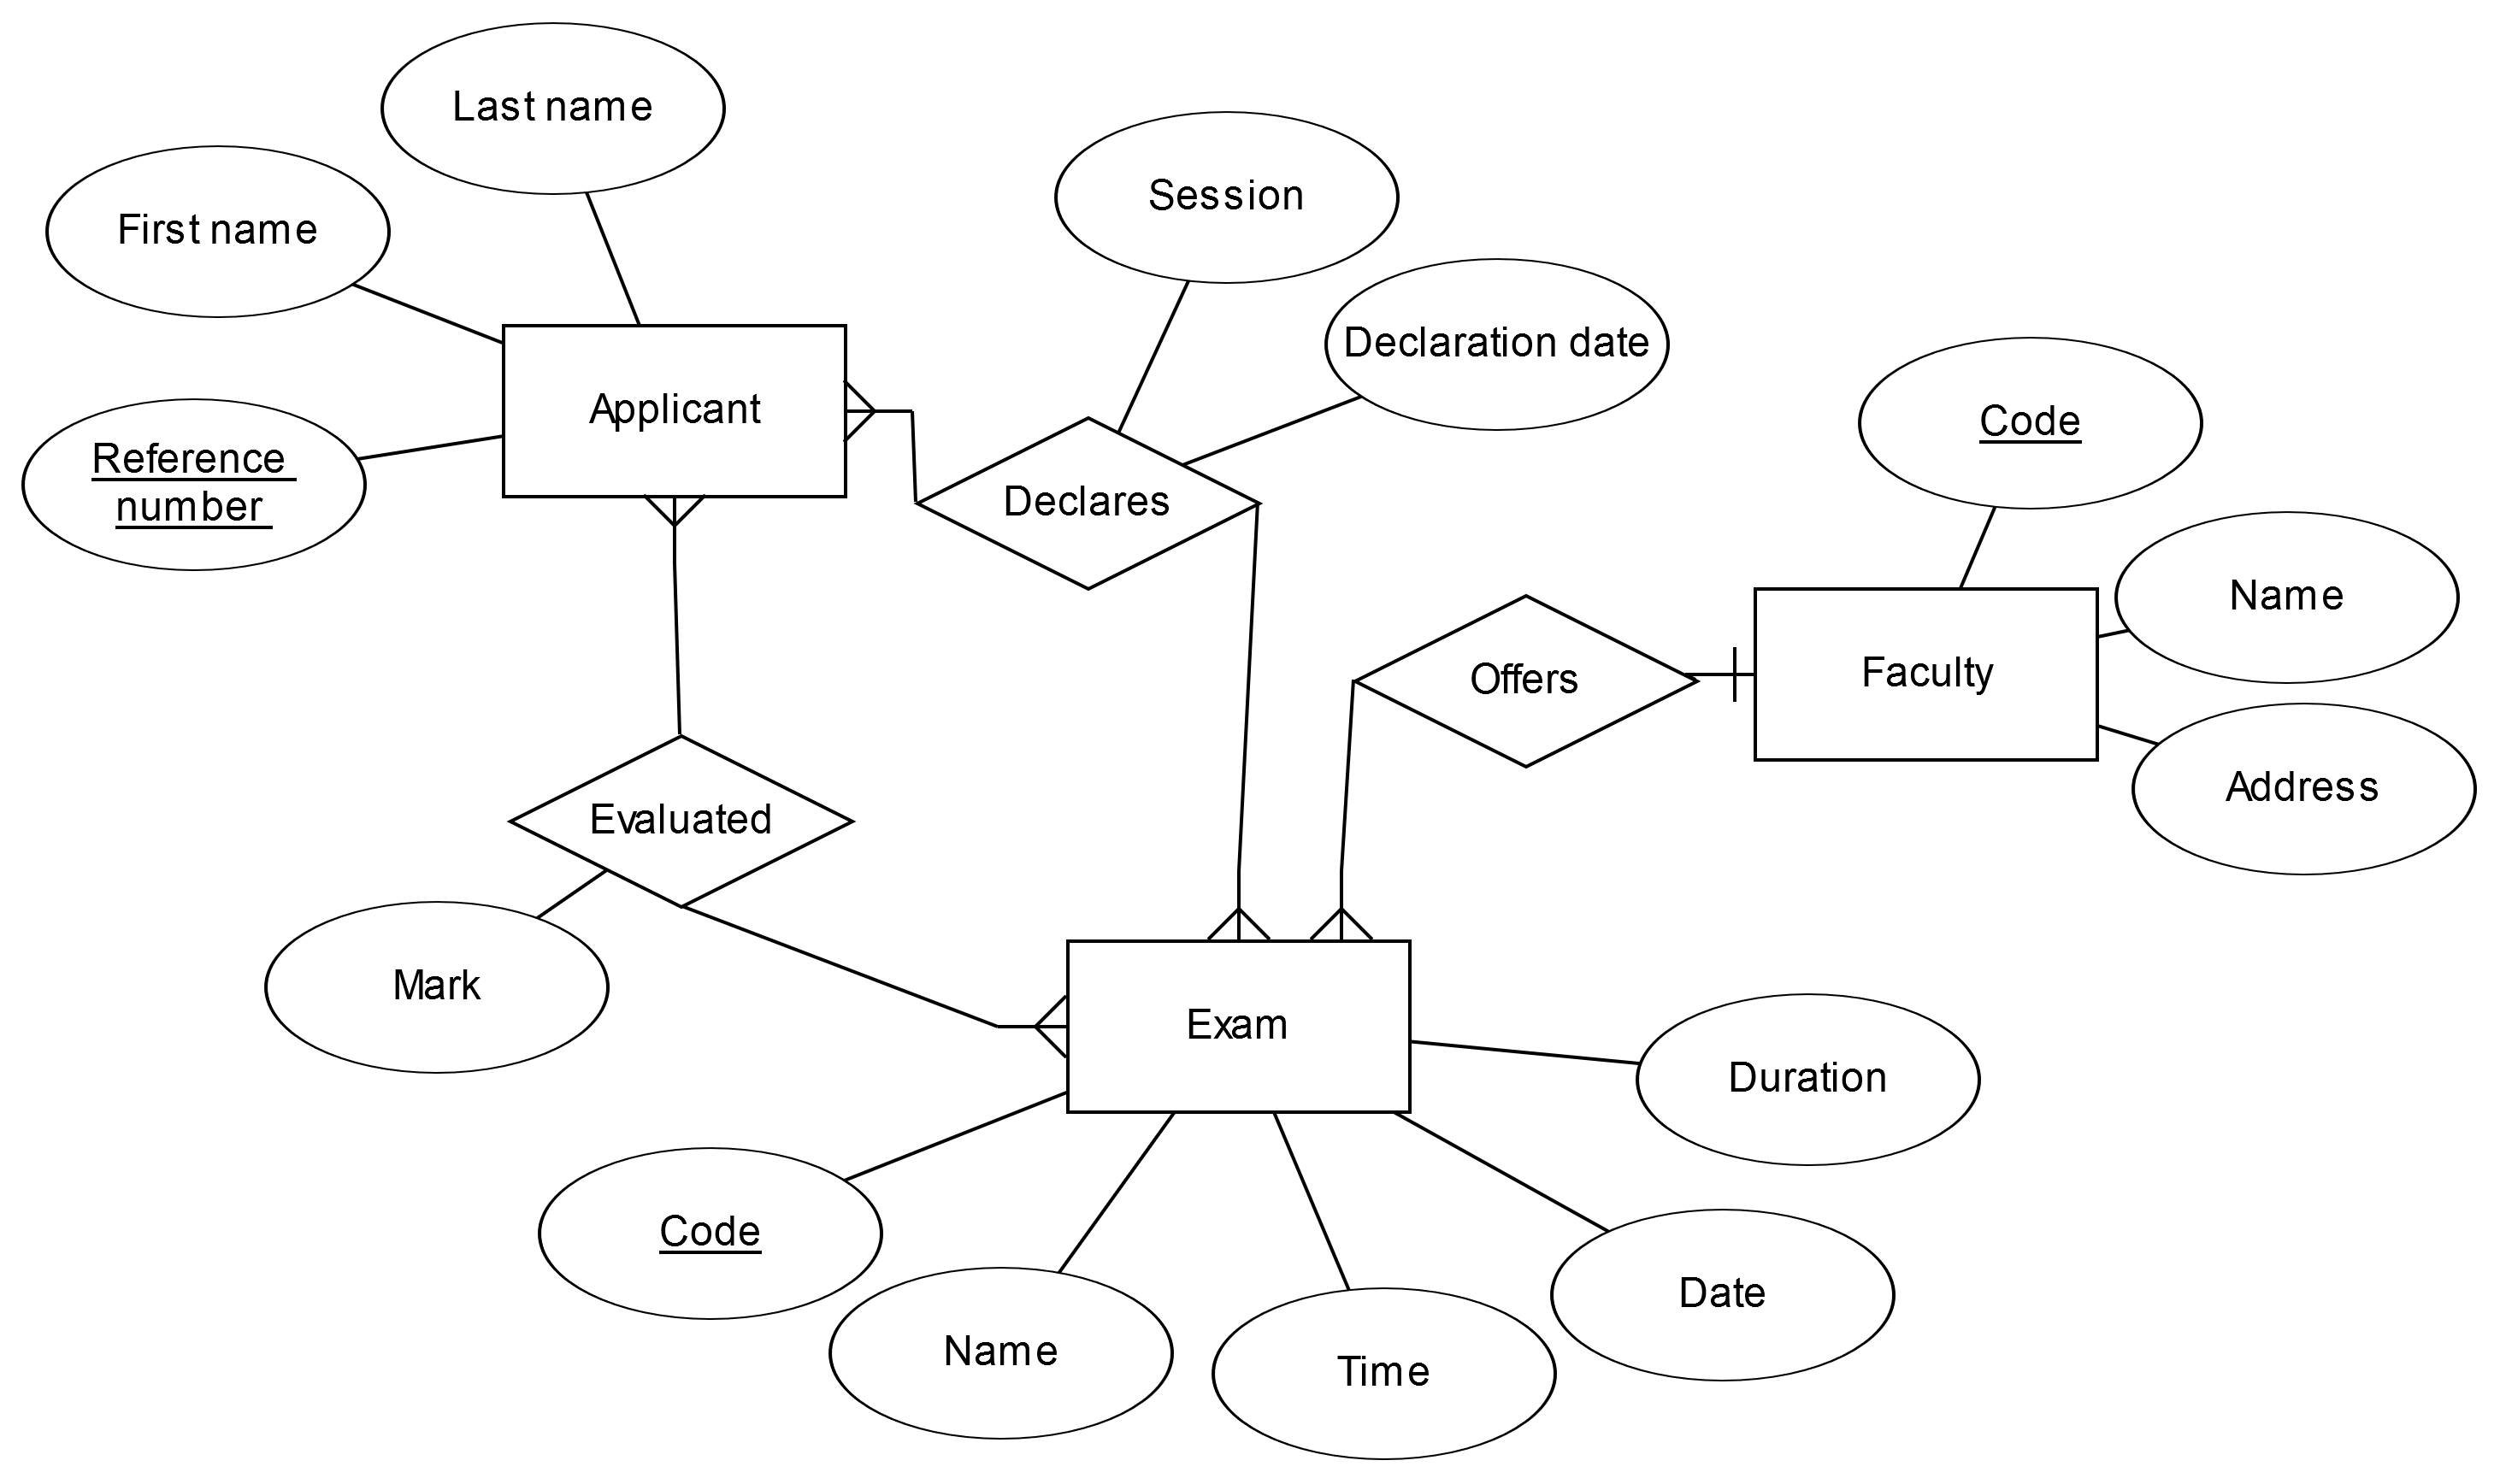
\includegraphics[width=1.30\textwidth]{er.png}
\caption{E\textbackslash R диаграма, представяща описания модел}
\end{figure}
\pagebreak

\section{Релационен модел}
Използвайки NULL подхода получаваме следните релации :\\
Person(\underline{PersonalNo}, Name, Salary);\\
Reader (\underline{ReaderId}, RegistrationDate, ExpirationDate);\\
Fines(\underline{FineNo}, Value, PaymentDate);\\
Book(\underline{SystemNo}, ISBN, Title, Pages, Edition, Type);\\
Publisher(\underline{PublisherID}, Name, Address);\\
Department(\underline{DepNo}, Name, Address);\\
Registered(\underline{PersonalNo}, \underline{ReaderID});\\
Superior(\underline{PersonalNo}, \underline{SuperiorPersonalNo};\\
WorksIn(\underline{PersonalNo}, \underline{DepNo}, Position);\\
WrittenBy(\underline{SystemNo}, \underline{PersonalNo});\\
Borrows(\underline{ReaderID}, \underline{SystemNo}, \underline{BorrowDate}, DueDate, ReturnDate),\\
PublishedBy(\underline{SystemNo}, \underline{PublisherID});\\
Location(\underline{DepNo}, \underline{SystemNo});\\
Has(\underline{ReaderID}, \underline{FineNo}, Value, PaymentDate).\\
\par
Забелязваме, че WorksIn, Has, Superior и PublishedBy са от вида много - един, поради което оптимизираме релационния модел, и получаваме:\\
Person(\underline{PersonalNo}, Name, Salary, SuperiorPersonalNo, DepNo, Position);\\
Reader(\underline{ReaderID}, RegistrationDate, ExpirationDate);\\
Fines(\underline{FineNo}, Value, PaymentDate, ReaderID);\\
Book(\underline{SystemNo}, ISBN, Title, Pages, Edition, Type, PublisherID, PublishDate);\\
Publisher(\underline{PublisherID},  Name, Address);\\
Department(\underline{DepNo},  Name, Address);\\
Registered(\underline{PersonalNo}, \underline{ReaderID});\\
WrittenBy(\underline{SystemNo}, \underline{PersonalNo});\\
Borrows(\underline{ReaderID}, \underline{SystemNo}, \underline{BorrowDate}, DueDate, ReturnDate);\\
Location(\underline{DepNo}, \underline{SystemNo}).\\

\par Във всяка една от релациите, компонентите са атомарни, което означава че всички релации са в 1НФ. Търсим функционални зависимости с цел да нормализираме получения релационен модел, ако е необходимо: 
\begin{enumerate}
\item Person:
\begin{itemize}
\item \textit {PersonalNo $\rightarrow$ Name, Salary, SuperiorPersonalNo, DepNo, Position}
\item \textit {PersonalNo, Name, DepNo, Position $\rightarrow$ Salary, SuperiorPersonalNo}
\item \textit {PersonalNo, DepNo, Position $\rightarrow$ Name, Salary, SuperiorPersonalNo}
\end{itemize}
\par
За да е релацията в 2НФ, то всеки атрибут трябва да е функционално зависим от атрибутите, съставляващи първичния ключ, но не и от негово подмножество. В частност първичния ключ на тази релация се състои от един елемент и единственто възможно подмножесто е празното, което не определя никой атрибут. За 3НФ е необходима 2НФ и ако A1, A2, ..An->B е нетривиална ФЗ която е в сила за R, то или \{A1, A2, ..An\} да е супер-ключ за R или B да е част от ключ. В случая и двете условия са изпълнени, т.е. нашата релация е в 3НФ.

\item Reader:
\begin{itemize}
\item \textit{ReaderID $\rightarrow$ RegistrationDate, ExpirationDate}
\item \textit{ReaderID, RegistrationDate $\rightarrow$ ExpirationDate}
\end {itemize}
\par
Аргументите, които важат за предишната релация Reader, са валидни и за тази.

\item Fines:
\begin{itemize}
\item \textit{FineNo $\rightarrow$ Value, PaymentDate, ReaderID}
\item \textit{FineNo, ReaderID $\rightarrow$ Value, PaymentDate}
\item \textit{FineNo, ReaderID, Value $\rightarrow$ PaymentDate}
\end {itemize}
И тук, както в предните два случая можем да приложим същите аргументи и да заключим, че релацията е в 3НФ.

\item Book:
\begin{itemize}
\item \textit{SystemNo $\rightarrow$ ISBN, Title, Pages, Edition, Type, PublisherID, PublishDate,Taken}
\item \textit{ISBN $\rightarrow$ Title, Pages, Edition, Type, PublisherID, PublishDate}
\end{itemize}
Въпреки, че релацията е в 2НФ, втората функционална зависимост нарушава правилото за 3НФ и затова се налага да нормализираме. В резултат на нормализацията получаваме следните две релации, които са в 3НФ:\\
Inventory(\underline{SystemNo}, ISBN,Taken),
Book(\underline{ISBN}, Title, Pages, Edition, Type, PublisherID, PublishDate)

\item Publisher:
\begin{itemize}
\item \textit{PublisherID $\rightarrow$ Name, Address}
\item \textit{PublisherID, Name $\rightarrow$ Address}
\item \textit{Name, Address $\rightarrow$ PublisherID}
\end{itemize}
Отново, както и в релацията Person можем да видим, че релацията е в 3НФ, като разликата тук е, че в последната функционална зависимост дясната страна е част от ключ.

\item Department:
Следваме същата логика както за предишната релация - няма нужда да правим нормализация.

\item Registered, WrittenBy:
Тъй като и двете релации съдържат само по два атрибута то те са в НФБК. Единствената промяна, която ще направим е да подменим атрибута SystemNo с ISBN за да избегнем повторения (може да има много книги с един и същ ISBN, но различини SystemNo).

\item Borrows:
\begin{itemize}
\item \textit{ReaderID, SystemNo $\rightarrow$ BorrowDate, DueDate, ReturnDate}
\item \textit{ReaderID, SystemNo, BorrowDate $\rightarrow$ DueDate, ReturnDate}
\item \textit {ReaderID, SystemNo, ReturnDate $\rightarrow$ BorrowDate, DueDate}
\end{itemize}
В случая всеки атрибут зависи от ReaderID и SystemNo, но поотделно нито читател, нито книга определят заемане, т.е. имаме 2НФ. За всяка от посочените ФЗ, лявата част е суперключ, следователно имаме 3НФ и не се налага да нормализираме.
\item Location:
\begin{itemize}
\item \textit { SystemNo $\rightarrow$ DepNo}
\end{itemize}
Тук ключът е \{DepNo, SystemNo\} и очевидно релацията е в 2НФ, а понеже и функционалната зависимост удовретворява условието дясната страна да е част от ключ, то релацията е в 3НФ.
\end{enumerate} 

На фигура 2 е илюстриран релационен модел, описващ базата данни.
\pagebreak

\begin{figure}[h!]
\hspace{-70pt}
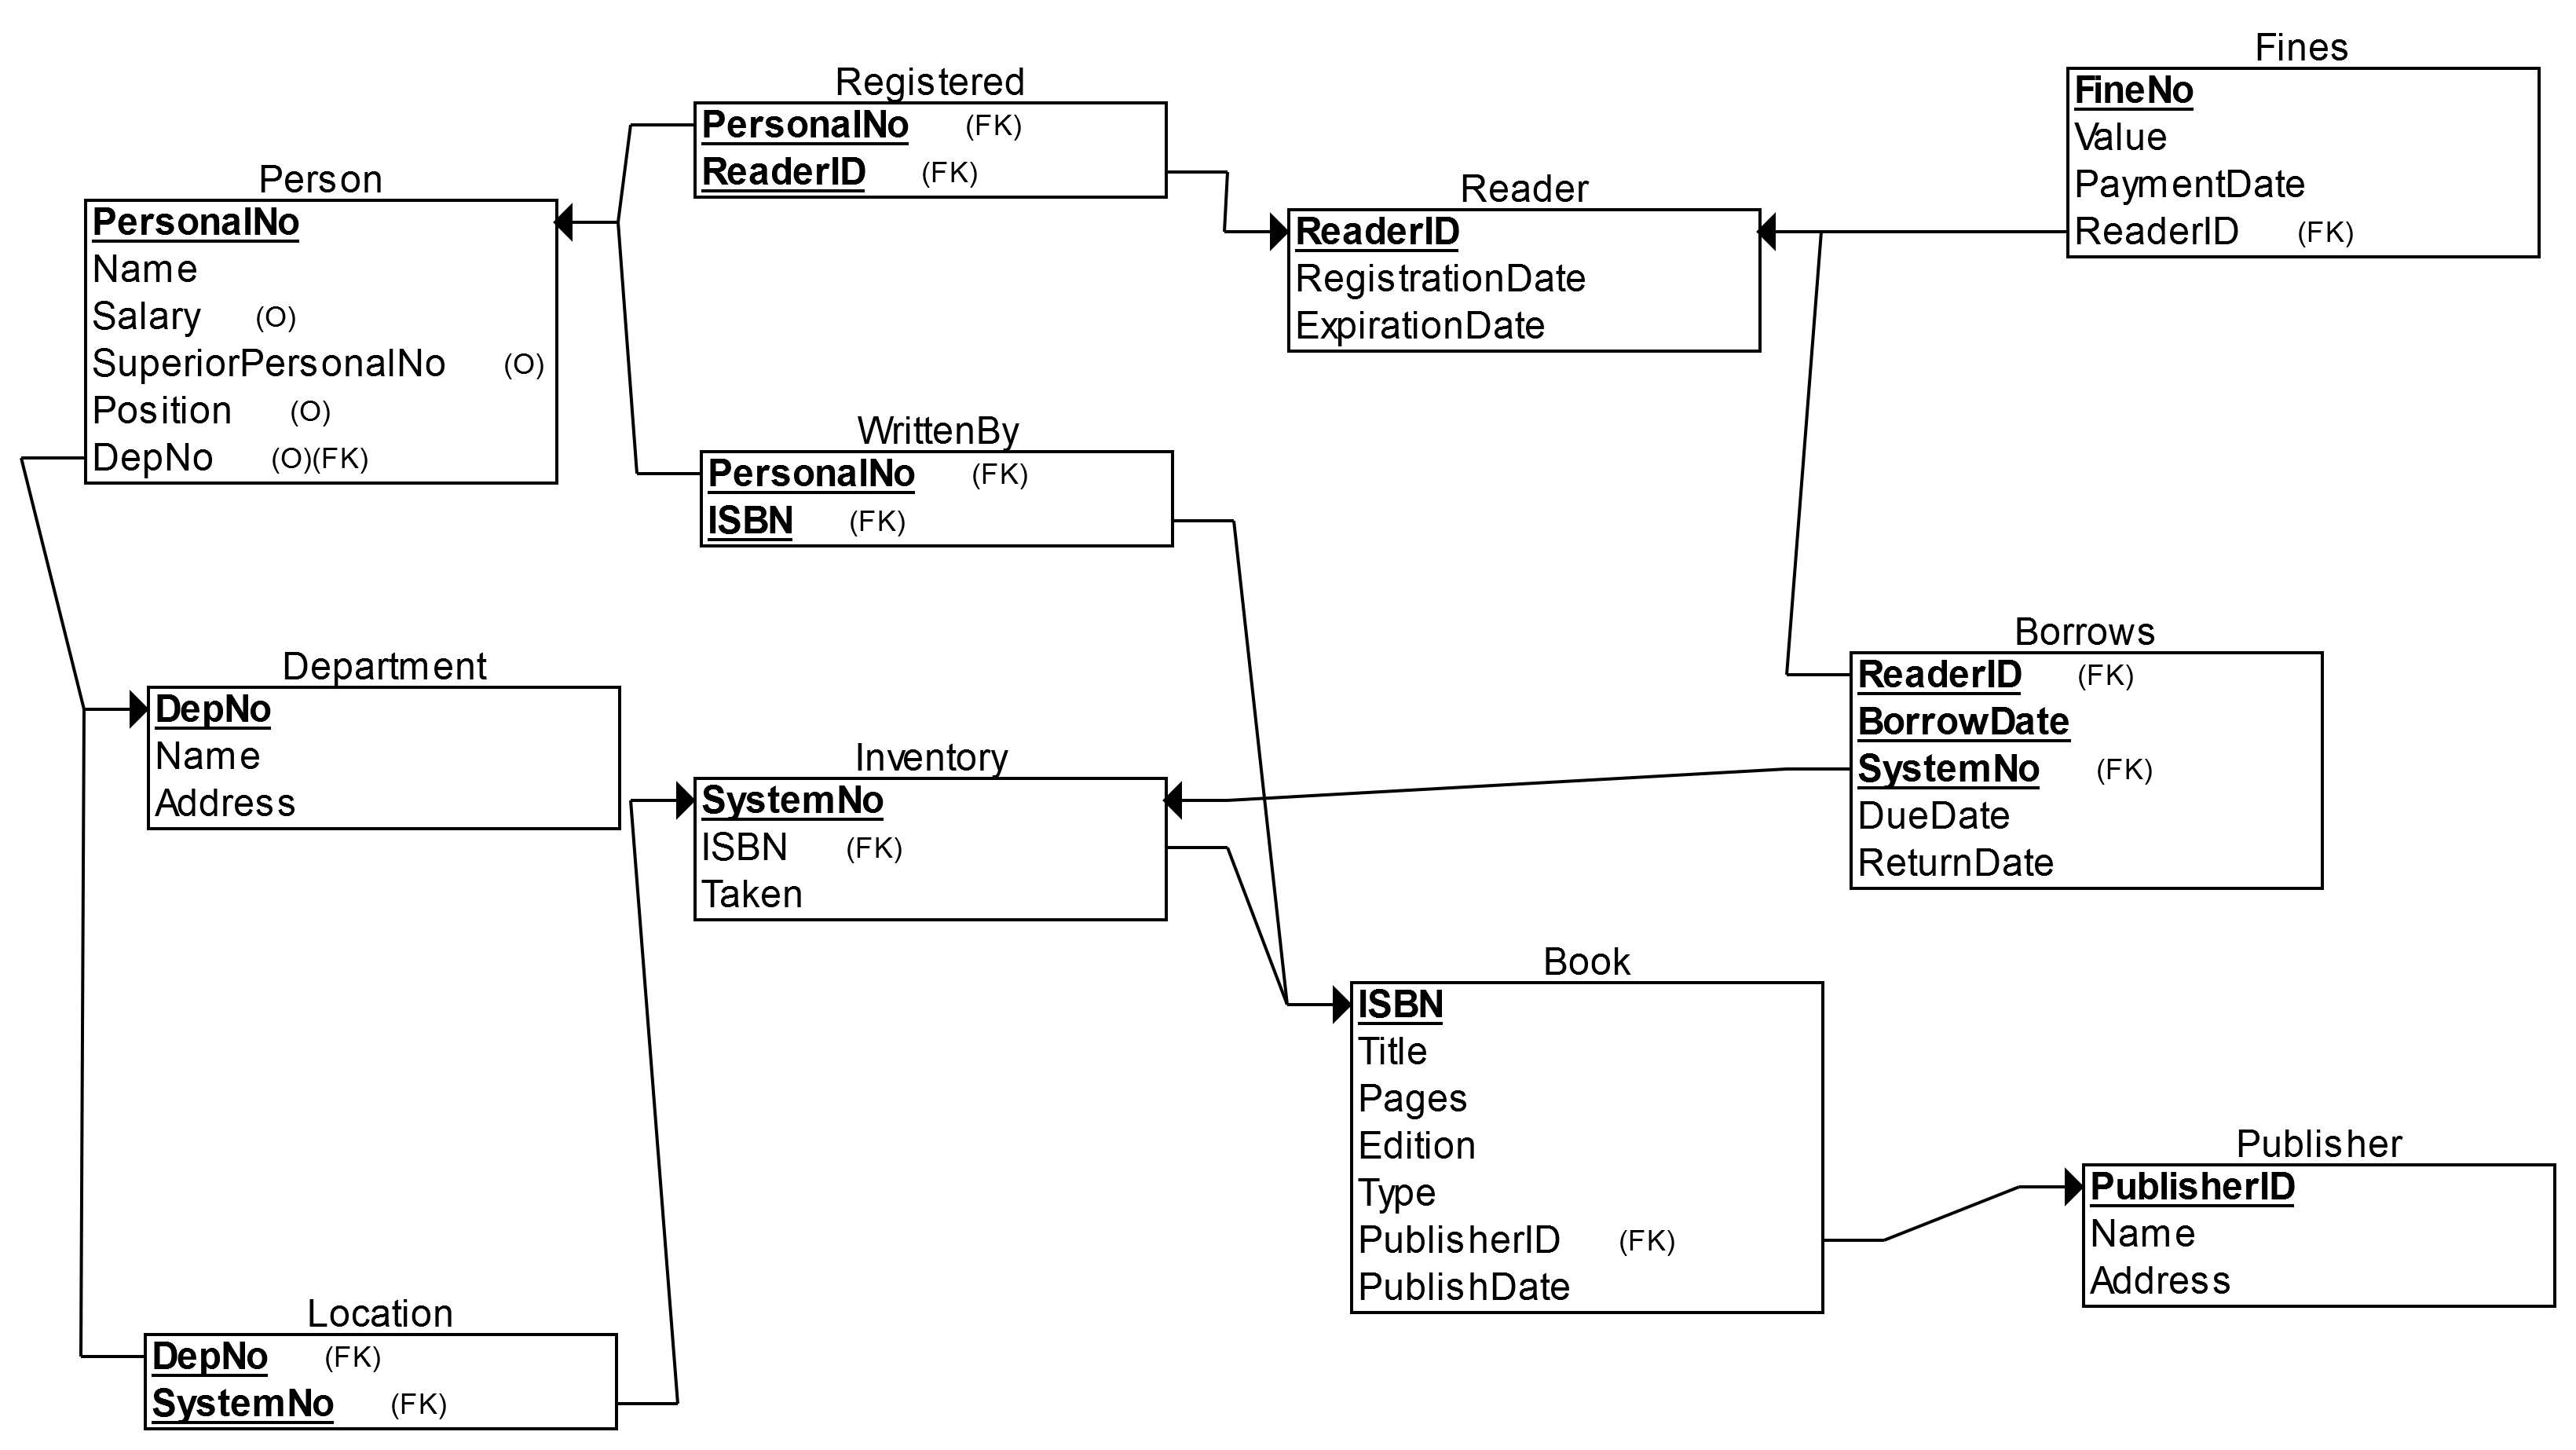
\includegraphics[width=1.30\textwidth]{relational.png}
\caption{Релационен модел на базата данни}
\end{figure}
\pagebreak

\section {Функции}
Дефинирани са четири функции: most\textunderscore read, register\textunderscore person, \\dep\textunderscore contains\textunderscore isbn, borrow\textunderscore book.
\par 
Функцията  most\textunderscore read не приема никакви параметри и връща ISBN-а на книгата, която е била заемана най - често от всички книги (независимо от кой клон на библиотеката). 
\par
Функцията register\textunderscore person приема два параметъра - низ от 10 символа съдържащ personalNo и цяло число, което означава идентификатора на новия читател. Функцията регистрира нов читател с посочените параметри и връща true ако действието е било успешно. Ако вече съществува читател с подадения идентификатор или не съществува човек,чиито номер да отговаря на подадения, то функцията хвърля изключение.
\par
Dep\textunderscore contains\textunderscore isbn e функция, която приема два параметъра и връща стойност от булев тип. Двата параметъра означават съответно ISBN на книга и номер на клон на библиотеката, като съответно типът на първата променлива е char(13), а на втората int. При некоректни параметри(т.е. не съществуащ клон или книга с посочения ISBN), функцията връща информация за настъпилото изключение, а в противен случай връща стойност, която зависи от това дали съответната книга може да бъде намерана в искания клон.
\par
Последната дефинирана функция borrow\textunderscore book приема три параметъра - идентификатор на читател, ISBN на книга и номер на клон, а връща променлива от тип varchar(255), която означава системен номер на книга. Целта на функцията е да заеме първата свободна книга, чиито ISBN и клон отговарят на изисканите и да върне нейният системен номер. Отново при некоректни параметри функцията дава на потребителя информация за настъпилото изключение.
\section {Тригери}
Във файлът createTrig.sql са дефинирани следните два тригера : trigger \textunderscore ins\textunderscore borrow и trigger \textunderscore publisher \textunderscore book. 
\par
Първият тригер - \textunderscore ins\textunderscore borrow се изпълнява след добавяне на нов запис в таблицата Borrows. Той се грижи за отбелязването на книгата, отговаряща на новодобавения запис, като взета в таблицата Inventory.
\par
Тригерът trigger \textunderscore publisher \textunderscore book се активира след добавяне на запис в таблицата Book. При своето изпълнение, ако не съществува издателство с необходимия идентификатор в таблицата Publisher, той добавя ново издателство, без формално име и адрес, за да запази валидността на външния ключ.
\section {Изгледи}
Трите изгледа: not\textunderscore returned, authorsbooks и publisher\textunderscore books са дефинирани във файла createView.sql.
\par
Изгледът not\textunderscore returned връща всички книги, които са взети и все още не върнати, т.е. имат отбелязан статус taken в таблицата Inventory. Информацията, която се връща е системния номер на книгата, идентификатор на читателя и краен срок за връщане.
\par
Authorsbooks е изглед дефиниран така, че да ни връща инфирмация за това, коя книга от кого е написана - връщат се ISBN, име на книгата и автор, където за всяка уникална двойка (произведение, автор) се среща по един запис.
\par
Последният дефиниран изглед - publisher\textunderscore books ни връща информация за това коя книга от кое издателство е - връщат се ISBN, заглавие, име на издателство, което отговаря за издаването на книгата и дата на издаване.
\section {Приложение за достъп до базата данни}
Приложението за достъп до базата данни е написано на Java и работи по следния начин : При стартиране потребителят трябва да въведе хоста, порта, на който работи базата данни, името на базата данни, credentials за достъп до базата и schema. След това той има избор от критерии, по които може да търси книга - ISBN, име, автор, издателство или системен номер. След като направи избор, потребителят въвежда низ, по който низ, както и по избрания критерии, той получава отговор на своята заявка. На фиг.3 са показани примерни резултати при изпълнение на заявки, като базата данни е попълнена с информация от скрипта dataLoad.sql.\\
\begin{figure}[]
\hspace{-70pt}
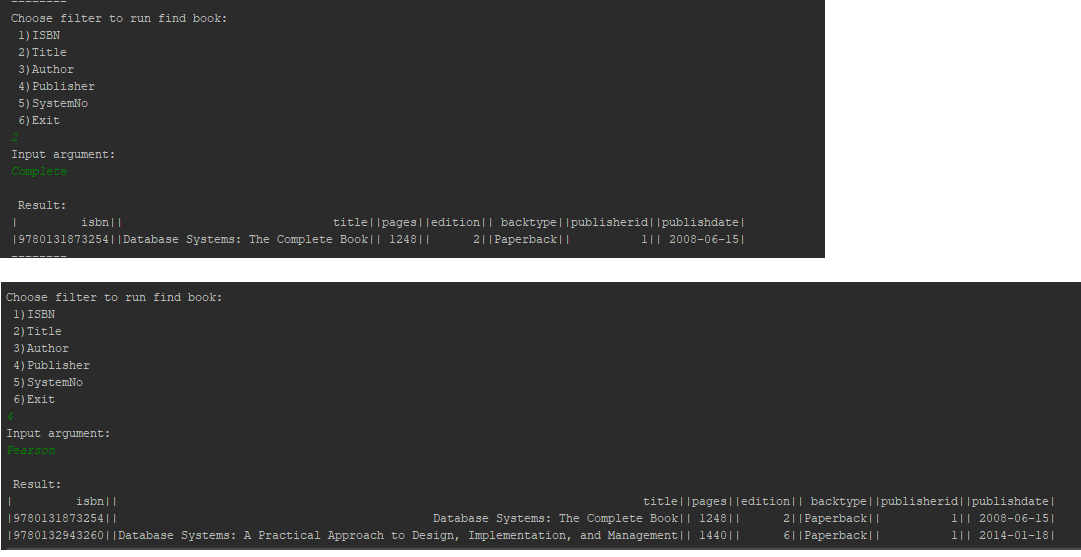
\includegraphics[width=1.30\textwidth]{app.png}
\caption{Примерни заявки, изпълнени от приложението}
\end{figure}
\\
\textbf{Забележка: } Скриптовете използвани при реализацията на проекта, както и примерното приложение са написани и тествани за PostgreSQL11 сървър. В зависимост от това дали се използва различна версия или различен сървър, може да възникнат проблеми при използването на скрипта и приложението.
\end{document}